
\documentclass[12pt,singleside,a4paper]{article}
\usepackage{float}
\usepackage[utf8]{inputenc}
\usepackage[T1]{fontenc}
\usepackage{mwe}
\usepackage{graphicx}
\usepackage{epsfig}
\usepackage{cite}
\usepackage{geometry}
\usepackage{float}
\usepackage{subfig}
\usepackage{comment}
\usepackage{listings}
\usepackage{xcolor}
\usepackage{pdfpages}
\usepackage[]{hyperref}

\definecolor{vgreen}{RGB}{104,180,104}
\definecolor{vblue}{RGB}{49,49,255}
\definecolor{vorange}{RGB}{255,143,102}


\lstdefinestyle{verilog-style}
{
    language=Verilog,
    frame=single,
    column=fullflexible,
    basicstyle=\small\ttfamily,
    keywordstyle=\color{vblue},
    identifierstyle=\color{black},
    commentstyle=\color{vgreen},
    moredelim=*[s][\colorIndex]{[}{]},
    literate=*{:}{:}1
}

\makeatletter
\newcommand*\@lbracket{[}
\newcommand*\@rbracket{]}
\newcommand*\@colon{:}
\newcommand*\colorIndex{%
    \edef\@temp{\the\lst@token}%
    \ifx\@temp\@lbracket \color{black}%
    \else\ifx\@temp\@rbracket \color{black}%
    \else\ifx\@temp\@colon \color{black}%
    \else \color{vorange}%
    \fi\fi\fi
}
\makeatother


\usepackage{trace}
\lstdefinelanguage{VHDL}{
   morekeywords=[1]{
     LIBRARY,USE,ENTITY,IS,PORT,IN,OUT,END,ARCHITECTURE,OF,
     BEGIN,DOWNTO,ALL, PROCESS, SIGNAL,COMPONENT, WAIT , FOR,WHEN, CASE 
   },
   morekeywords=[2]{
     STD_LOGIC_VECTOR,STD_LOGIC,IEEE,STD_LOGIC_1164,
     NUMERIC_STD,STD_LOGIC_ARITH,STD_LOGIC_UNSIGNED,std_logic_vector,AND,OR,NOT,NAND,NOR,XOR,
     std_logic
   },
   morecomment=[l]--
}
\usepackage[usenames,dvipsnames]{xcolor}
\colorlet{keyword}{blue!100!black!80}
\colorlet{STD}{red}
\colorlet{comment}{green!80!black!90}
\lstdefinestyle{VHDL}{
   language     = VHDL, 
   basicstyle   = \footnotesize \ttfamily,
   keywordstyle = [1]\color{keyword}\bfseries,
   keywordstyle = [2]\color{STD}\bfseries,
   commentstyle = \color{comment}
}

\usepackage[colorlinks]{hyperref}



\geometry{left=20mm,right=20mm,top=20mm,bottom=30mm}


\begin{document}
\begin{titlepage}
	\centering
    \textsc{\LARGE Seven Segment Display}\\[2.0 cm]
    
\begin{figure}[!htb]
\centering
  
\includegraphics[width=3cm,keepaspectratio]{logo.png}\textbf{  }\textbf{  }
  
\includegraphics[width=3cm,keepaspectratio]{download.png}\textbf{  }
  
\includegraphics[width=3cm,keepaspectratio]{modelsim-logo.jpg}
\end{figure}\\[1.0 cm]	
	\begin{minipage}{0.4\textwidth}
		\begin{flushleft} \large
			\emph{Mentors}\\
			Prasad Trimukhe\\
            Aditya Gudla\\
            Simranjeet Singh \
			\end{flushleft}
			\end{minipage}~
			\begin{minipage}{0.4\textwidth}
            
			\begin{flushright} \large
			\emph{Interns} \\
			Ajay Chaudhari\\
            Chethan T Bhat\\
            Ritvik Tiwari \\
            Karthik A Shet \\
		\end{flushright}
	\end{minipage}\\[2 cm]
\end{titlepage}
\pagenumbering{arabic}
\newpage
\tableofcontents
\newpage
\pagenumbering{arabic}
\section{Introduction}

\noindent The Seven Segment display has seven LEDs arranged into the number eight. They are both cost-effective and easy to use. The Figure 1 shows a standard seven-segment display.
\begin{center}
\begin{figure}[H]
    \centering
    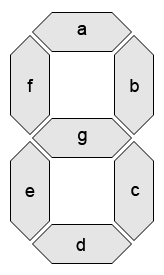
\includegraphics[scale=0.5]{Display/SevenLEDs.png}
    \caption{ Seven Segment Display }
\end{figure}
\end{center}
\noindent There are two types of seven-segment displays, \textbf{Common Anode} and \textbf{Common Cathode}. The Internal structure of both these types are identical except for the polarity of the LEDs and common terminal. The diagram below shows the internal structure of the common cathode seven-segment display(the one is used in this tutorial) and common anode seven-segment display.

\begin{figure}[H]
\centering
    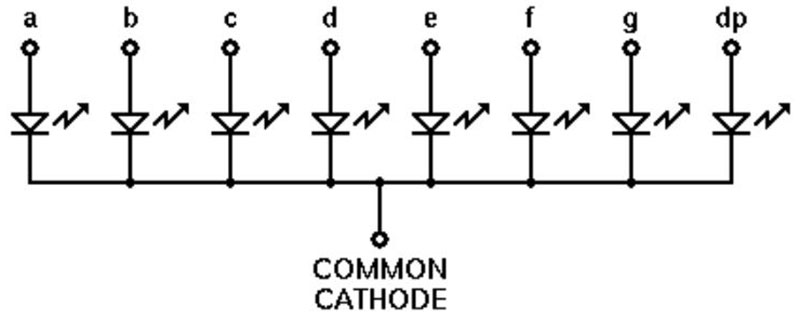
\includegraphics[scale=0.2]{Circuit/commoncathode.jpg}
    \caption{ Seven Segment Display with Common Cathode }
    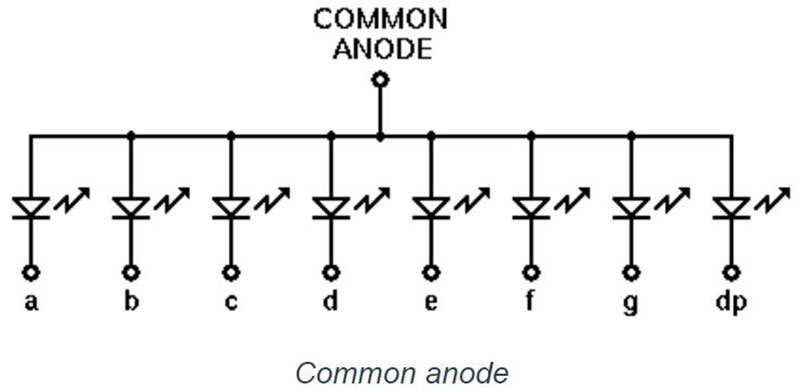
\includegraphics[scale=0.2]{Circuit/commonannode.jpg}
    \caption{ Seven Segment Display with Common Anode }
\end{figure}

\begin{itemize}
    \item The Common Cathode Display (CCD) – In the common cathode display, all the cathode connections of the LED’s are joined together to logic “0” or ground. The individual segments are illuminated by application of a “HIGH”, logic “1” signal to the individual Anode terminals.
    \item The Common Anode Display (CAD) – In the common anode display, all the anode connections of the LED’s are joined together to logic “1” and the individual segments are illuminated by connecting the individual Cathode terminals to a “LOW”, logic “0” signal.
\end{itemize} 
\noindent But, seven segment display does not work by directly supplying voltage to different segments of LEDs. First, our decimal number is changed to its BCD equivalent signal then the BCD to seven segment decoder converts that signals to the a suitable format which is then fed to seven segment display.
\\
\noindent  This BCD to seven segment decoder has four input lines (A, B, C and D) and 7 output lines (a, b, c, d, e, f and g), this output is given to seven segment LED display which displays the decimal number depending upon inputs.

\begin{center}
\begin{figure}[H]
    \centering
    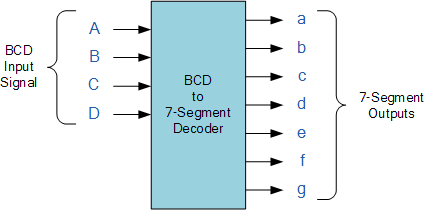
\includegraphics[scale=1]{Circuit/bcd.png}
    \caption{Design of BCD Decoder 4:7 }
\end{figure}
\end{center}





\begin{center}
\begin{tabular}{ |p{1cm}|p{1cm}|p{1.5cm}|p{1cm}|p{1cm}|p{1cm}|p{1cm}|p{1cm}|p{1cm}|p{1cm}|} \hline
 \multicolumn{10}{|c|}{Truth Table for Seven Segment Display}   \\ \hline \hline
    \textbf{NO.} &   \textbf{BCD}     &   \textbf{Display} &   \textbf{a}   &   \textbf{b}  &   \textbf{c}   &   \textbf{d}   &   \textbf{e}   &   \textbf{f}   &   \textbf{g}   \\ \hline
    0   &   0000    &    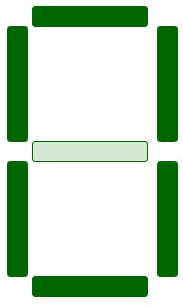
\includegraphics[scale=0.1]{Display/0.png}       &   1   &   1   &   1   &   1   &   1   &   1   &   0   \\\hline
    1   &   0001    &    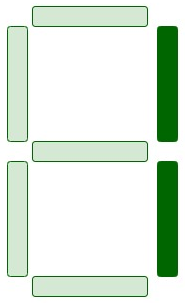
\includegraphics[scale=0.1]{Display/1.png}        &   0   &   1   &   1   &   0   &   0   &   0   &   0   \\\hline
    2   &   0010    &     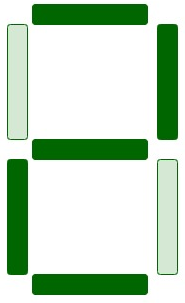
\includegraphics[scale=0.1]{Display/2.png}       &   1   &   1   &   0   &   1   &   1   &   0   &   1   \\\hline
    3   &   0011    &      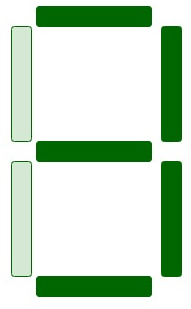
\includegraphics[scale=0.1]{Display/3.png}      &   1   &   1   &   1   &   1   &   0   &   0   &   1   \\\hline
    4   &   0100    &     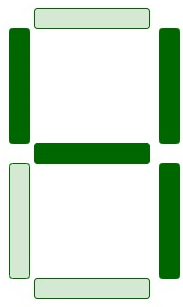
\includegraphics[scale=0.1]{Display/4.png}       &   0   &   0   &   1   &   0   &   0   &   1   &   1   \\\hline
    5   &   0101    &     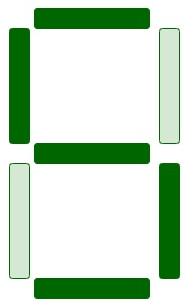
\includegraphics[scale=0.1]{Display/5.png}       &   1   &   0   &   1   &   1   &   0   &   1   &   1   \\\hline
    6   &   0110    &      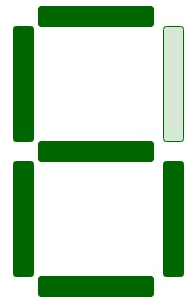
\includegraphics[scale=0.1]{Display/6.png}      &   1   &   0   &   1   &   1   &   1   &   1   &   1   \\\hline
    7   &   0111    &     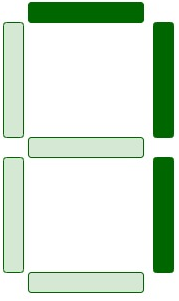
\includegraphics[scale=0.1]{Display/7.png}       &   1   &   1   &   1   &   0   &   0   &   0   &   0   \\\hline
    8   &   1000    &     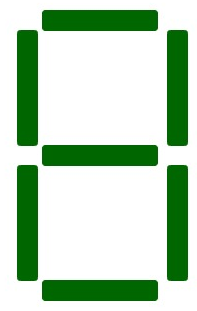
\includegraphics[scale=0.1]{Display/8.png}       &   1   &   1   &   1   &   1   &   1   &   1   &   1   \\\hline
    9   &   1001    &     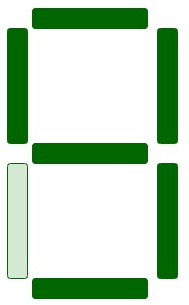
\includegraphics[scale=0.1]{Display/9.png}       &   1   &   1   &   1   &   1   &   0   &   1   &   1   \\\hline
    



\end{tabular} 
\captionof{table}{Truth Table for Seven Segment Display}
\end{center}



\newpage
\section{Code}
\subsection{VHDL code for Seven Segment Display }
\begin{lstlisting}[style=VHDL, frame=single,linewidth = 18cm]
-----------------------------------------------------------
-- File:    Seven_Segment_Display_VHDL.vhd
-- Description:	This is an implementation of a Seven Segment Display using a 
--          using Case Statement or behaviourial modelling
--	    Seven display consist of 7 led segments to display 0 to 6 which 
--	    will be named as  A to G.
--	    We will design a BCD to 7 Segment Decoder converts which converts 
--	    4 bit binary to 7 bit control signal which can be displayed on 
--	    7 segment display. 
-----------------------------------------------------------
-- Libraries
LIBRARY 	IEEE;
USE 		IEEE.STD_LOGIC_1164.ALL;
-- Entity Declaration
-- This is where all the Inputs & Outputs are specified, the BCD bit 
-- will be stored in BCDNos and 7 LEDs on the Segment are stored in DisplayLEDs
ENTITY Seven_Segment_Display_VHDL IS
    PORT(
		BCDNos		: IN STD_LOGIC_VECTOR  (3 DOWNTO 0);
		DisplayLEDs	: OUT STD_LOGIC_VECTOR (6 DOWNTO 0)
		);
	END Seven_Segment_Display_VHDL;
-- This is where we describe the behavior of the Seven Segment Display
ARCHITECTURE BEHAVIOURAL OF Seven_Segment_Display_VHDL IS
BEGIN
PROCESS(BCDNos)
    BEGIN
	CASE BCDNos IS
		WHEN "0000" =>
			DisplayLEDs <= "1111110"; ---0
		WHEN "0001" =>
			DisplayLEDs <= "0110000"; ---1
		WHEN "0010" =>
			DisplayLEDs <= "1101101"; ---2
		WHEN "0011" =>
			DisplayLEDs <= "1111001"; ---3
		WHEN "0100" =>
			DisplayLEDs <= "0010011"; ---4
		WHEN "0101" =>
			DisplayLEDs <= "1011011"; ---5
		WHEN "0110" =>
			DisplayLEDs <= "1011111"; ---6
		WHEN "0111" =>
			DisplayLEDs <= "1110000"; ---7
		WHEN "1000" =>
			DisplayLEDs <= "1111111"; ---8
		WHEN "1001" =>
			DisplayLEDs <= "1111011"; ---9
		WHEN others =>
			DisplayLEDs <= "0000000"; ---null
	END CASE;
	END PROCESS;
END BEHAVIOURAL;
 
\end{lstlisting} 
\subsection{ Verilog HDL code for Seven Segment Display }

\begin{lstlisting}[style =verilog-style,frame=single,linewidth = 18cm]
//Verilog code for sevent segment display
//Define module


module seven_segment(
	input [3:0]bcd,                     //Define all I/O ports
	output reg [6:0]display);


//Define Always block ,this block is executed every time the 
//input BCD value changes.
always @ (bcd)
begin
	case(bcd)
    4'b0000:display<=7'b1111110;//output port 'display' is assigned with  
    			//seven segment equivalent of input BCD (0)
    4'b0001:display<=7'b0110000;//output port 'display' is assigned with 
                                //seven segment equivalent of input BCD (1)
    4'b0010:display<=7'b1101101;//output port 'display' is assigned with  
                                //seven segment equivalent of input BCD (2)
    4'b0011:display<=7'b1111001;//output port 'display' is assigned with  
                                //seven segment equivalent of input BCD (3)
    4'b0100:display<=7'b0110011;//output port 'display' is assigned with  
                                //seven segment equivalent of input BCD (4)
    4'b0101:display<=7'b1011011;//output port 'display' is assigned with  
                                //seven segment equivalent of input BCD (5)
    4'b0110:display<=7'b1011111;//output port 'display' is assigned with  
                                //seven segment equivalent of input BCD (6)
    4'b0111:display<=7'b1110000;//output port 'display' is assigned with  
                                //seven segment equivalent of input BCD (7)
    4'b1000:display<=7'b1111111;//output port 'display' is assigned with 
                                //seven segment equivalent of input BCD (8)
    4'b1001:display<=7'b1111011;//output port 'display' is assigned with 
                                //seven segment equivalent of input BCD (9)
    default: display<=7'b0000000;
	
	endcase										//end of case block
end												//end of always block
endmodule										//end of module
\end{lstlisting}

\newpage
\section*{Test Bench Code}
\subsection{VHDL Test Bench code for Seven Segment Display }
\begin{lstlisting}[style=VHDL, frame=single,linewidth = 18cm]
-- Libraries
LIBRARY 	IEEE;
USE 		IEEE.STD_LOGIC_1164.ALL;
 
ENTITY Seven_Segment_Display_TB IS
END Seven_Segment_Display_TB;

ARCHITECTURE BEHAVIOURAL OF Seven_Segment_Display_TB IS
 
-- Component Declaration for the Unit Under Test (UUT) 
COMPONENT Seven_Segment_Display_VHDL
	PORT(   BCDNos		: IN STD_LOGIC_VECTOR  (3 DOWNTO 0);
			DisplayLEDs	: OUT STD_LOGIC_VECTOR (6 DOWNTO 0)
			);
	END COMPONENT;

SIGNAL BCDNos       : STD_LOGIC_VECTOR  (3 DOWNTO 0);   --INPUT BCD NO
SIGNAL DisplayLEDs : STD_LOGIC_VECTOR   (6 DOWNTO 0);	--OUTPUT LED SIGNAL
 
BEGIN
-- Initiate the Unit Under Test (UUT)
		uut: Seven_Segment_Display_VHDL PORT MAP (
	 			BCDNos 		=> BCDNos,
				DisplayLEDs => DisplayLEDs
				);
-- Stimulus process
		Stimulus_Process: PROCESS
		BEGIN
			BCDNos <= "0000";
				WAIT FOR 100 ns;
			BCDNos <= "0001";
				WAIT FOR 100 ns;
			BCDNos <= "0010";
				WAIT FOR 100 ns;
			BCDNos <= "0011";
				WAIT FOR 100 ns;
			BCDNos <= "0100";
				WAIT FOR 100 ns;
			BCDNos <= "0101";
				WAIT FOR 100 ns;
			BCDNos <= "0110";
				WAIT FOR 100 ns;
			BCDNos <= "0111";
				WAIT FOR 100 ns;
			BCDNos <= "1000";
				WAIT FOR 100 ns;
			BCDNos <= "1001";
				WAIT FOR 100 ns;
				WAIT;
	END PROCESS;
END BEHAVIOURAL;
\end{lstlisting}
\newpage
\subsection{Verilog HDL Test Bench code for Seven Segment Display }
\begin{lstlisting}[style =verilog-style,frame=single,linewidth = 18cm]
// Verilog code for test bench of sevensegment
//Define module 
module tb_seven_segment;


reg [3:0]bcd; reg clk;		//Define the input 	
wire [6:0]display;			//Define the outputs

//Map the I/O ports with UUT
seven_segment uut(.bcd(bcd),.display(display));     


// Define Initial block
initial begin				
        bcd=4'b0000;        //Initialise the input 'bcd' value to '0'
end



//Initialize input ports with different combination of BCD data
initial begin								
	bcd = 4'b0001;#100;
	bcd = 4'b0011;#100;
	bcd = 4'b1000;#100;
	bcd = 4'b1001;#100;
	#100;
end				//end of initial block.
endmodule			//end of module.
\end{lstlisting}
\newpage
\section{Implementing on quartus II}
 
For in-depth guide for creating a \textbf{New Project} follow \textbf{Quick Start Guide For Quartus Prime Lite Software}. Both Verilog HDL and VHDL code is provided in this tutorial, hence continue the tutorial by selecting only one language to avoid confusion.

\begin{enumerate}
    \item Create a \textbf{New Project} with the following settings
    \begin{figure}[H]
    \centering
    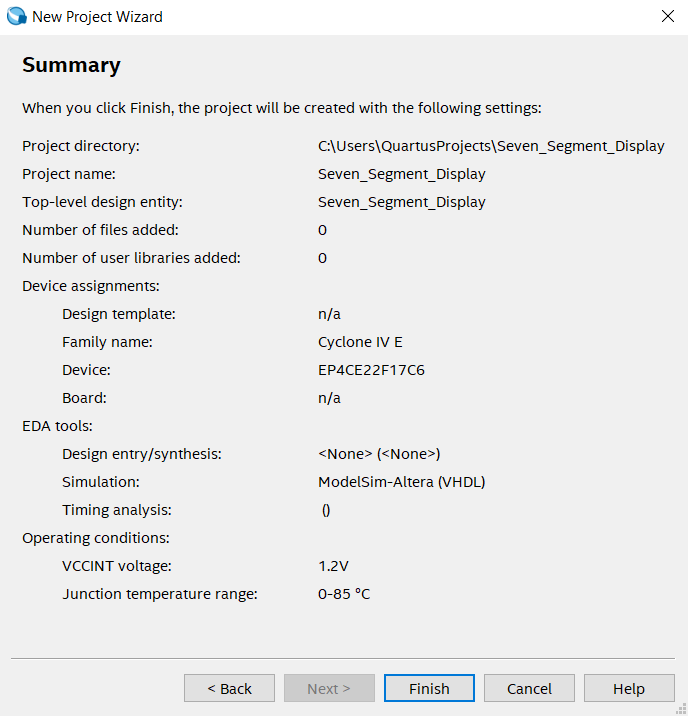
\includegraphics[width=9cm,keepaspectratio]{Project/Create1.png}
    \caption{Project Setting}
    \end{figure}

    \item Create a \textbf{New VHDL file}. As we will be demonstrating using VHDL code so select VHDL file. Use the code for Seven Segment Display mention above in the code section in this document.
    \begin{figure}[H]
    \centering
    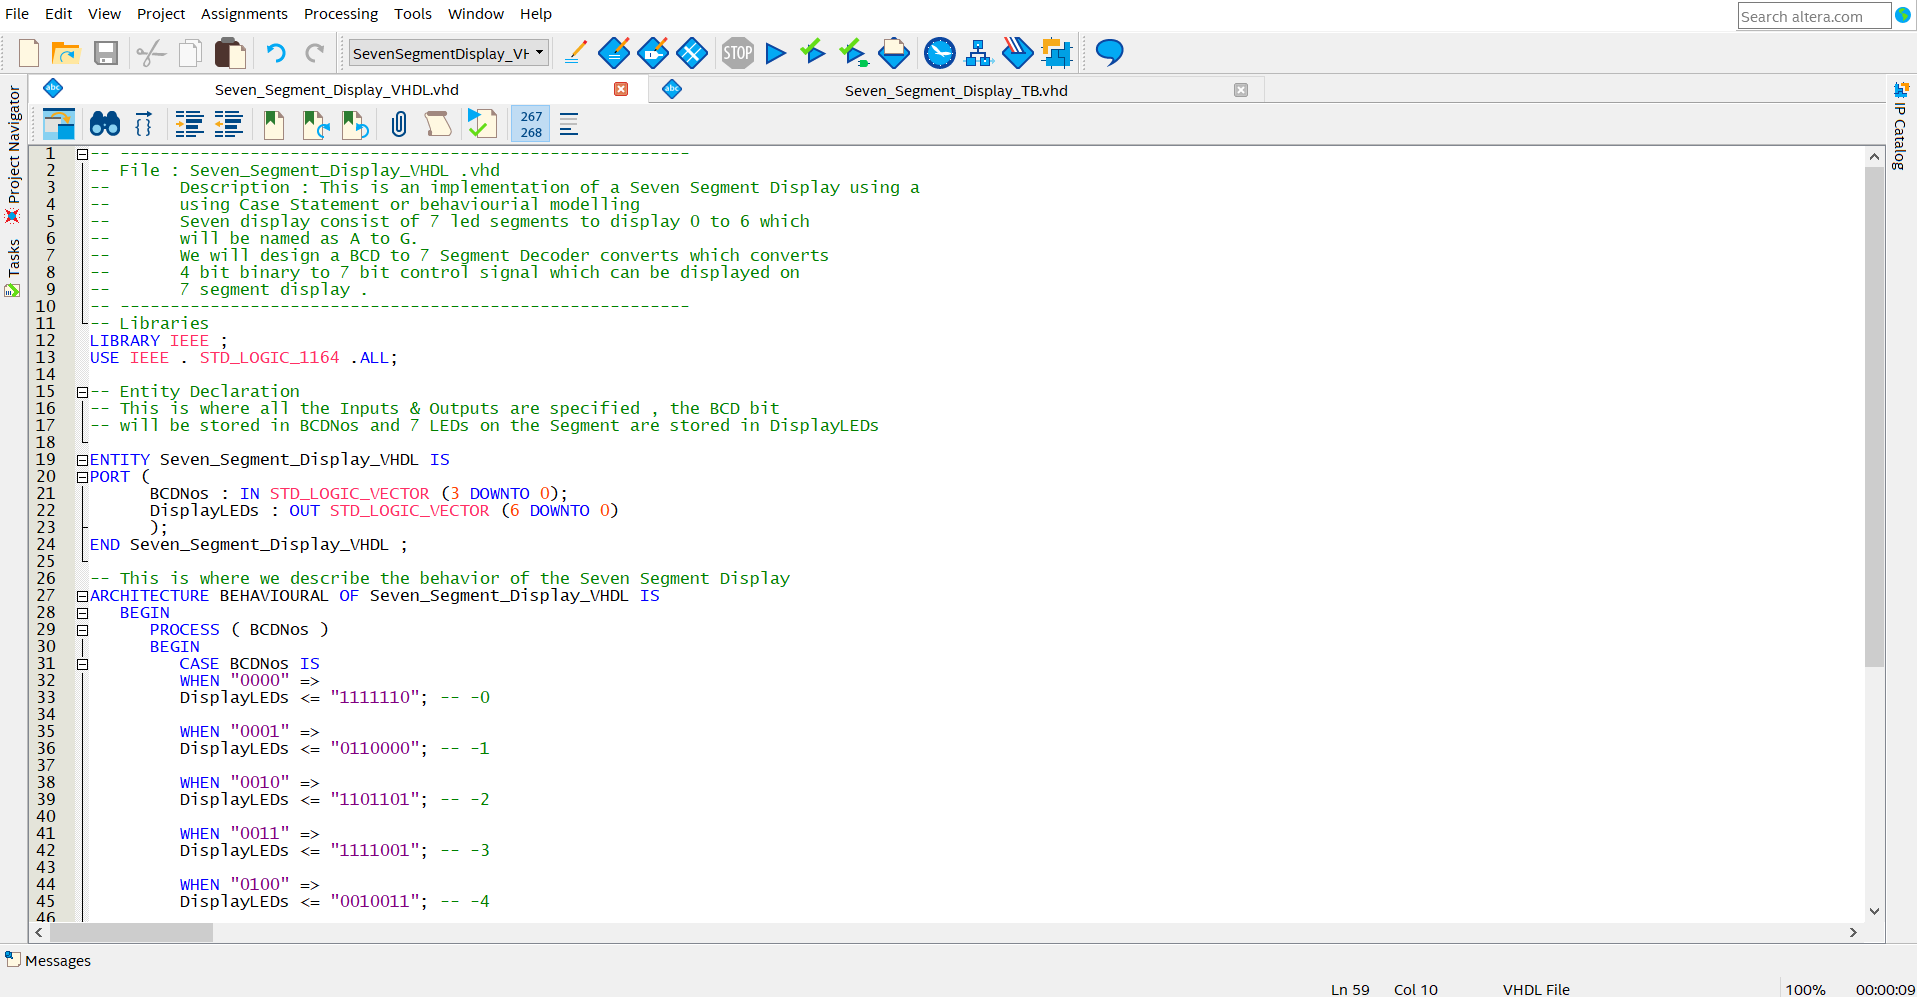
\includegraphics[width=12cm,keepaspectratio]{Project/vhdl.png}
    \caption{Create a VHDL file}
    \end{figure}
    \newpage
    
    
    \item Go to \textbf{File}$\rightarrow$\textbf{Save as}. Enter the Name of file (it should be same as module/entity name), Enter correct file extension, for VHDL it is \textbf{.vhd} and for Verilog HDL it is \textbf{.v } and then Click on \textbf{Save}
    \begin{figure}[H]
    \centering
    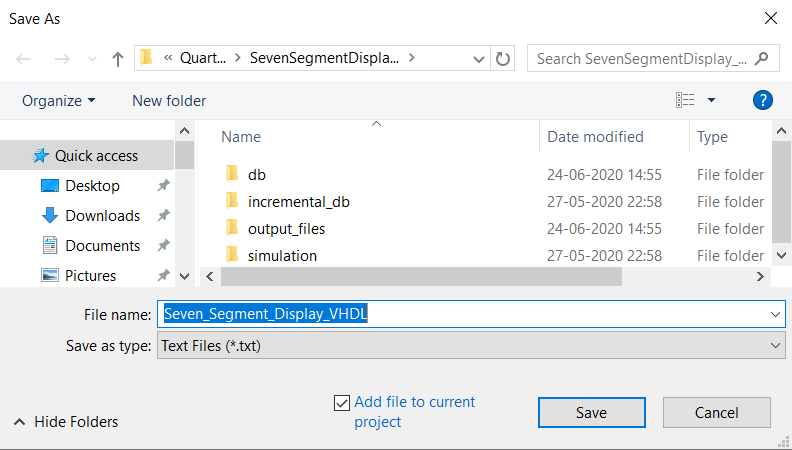
\includegraphics[width=14cm,keepaspectratio]{Project/Create3.png}
    \caption{Save the file}
    \end{figure}
    
    \item Goto \textbf{Project}$\rightarrow$\textbf{Set as Top-Level Entity}. The Seven\_Segment\_SDisplay file is our main file and make sure you have selected this file while setting the top level entity.
    \begin{figure}[H]
    \centering
    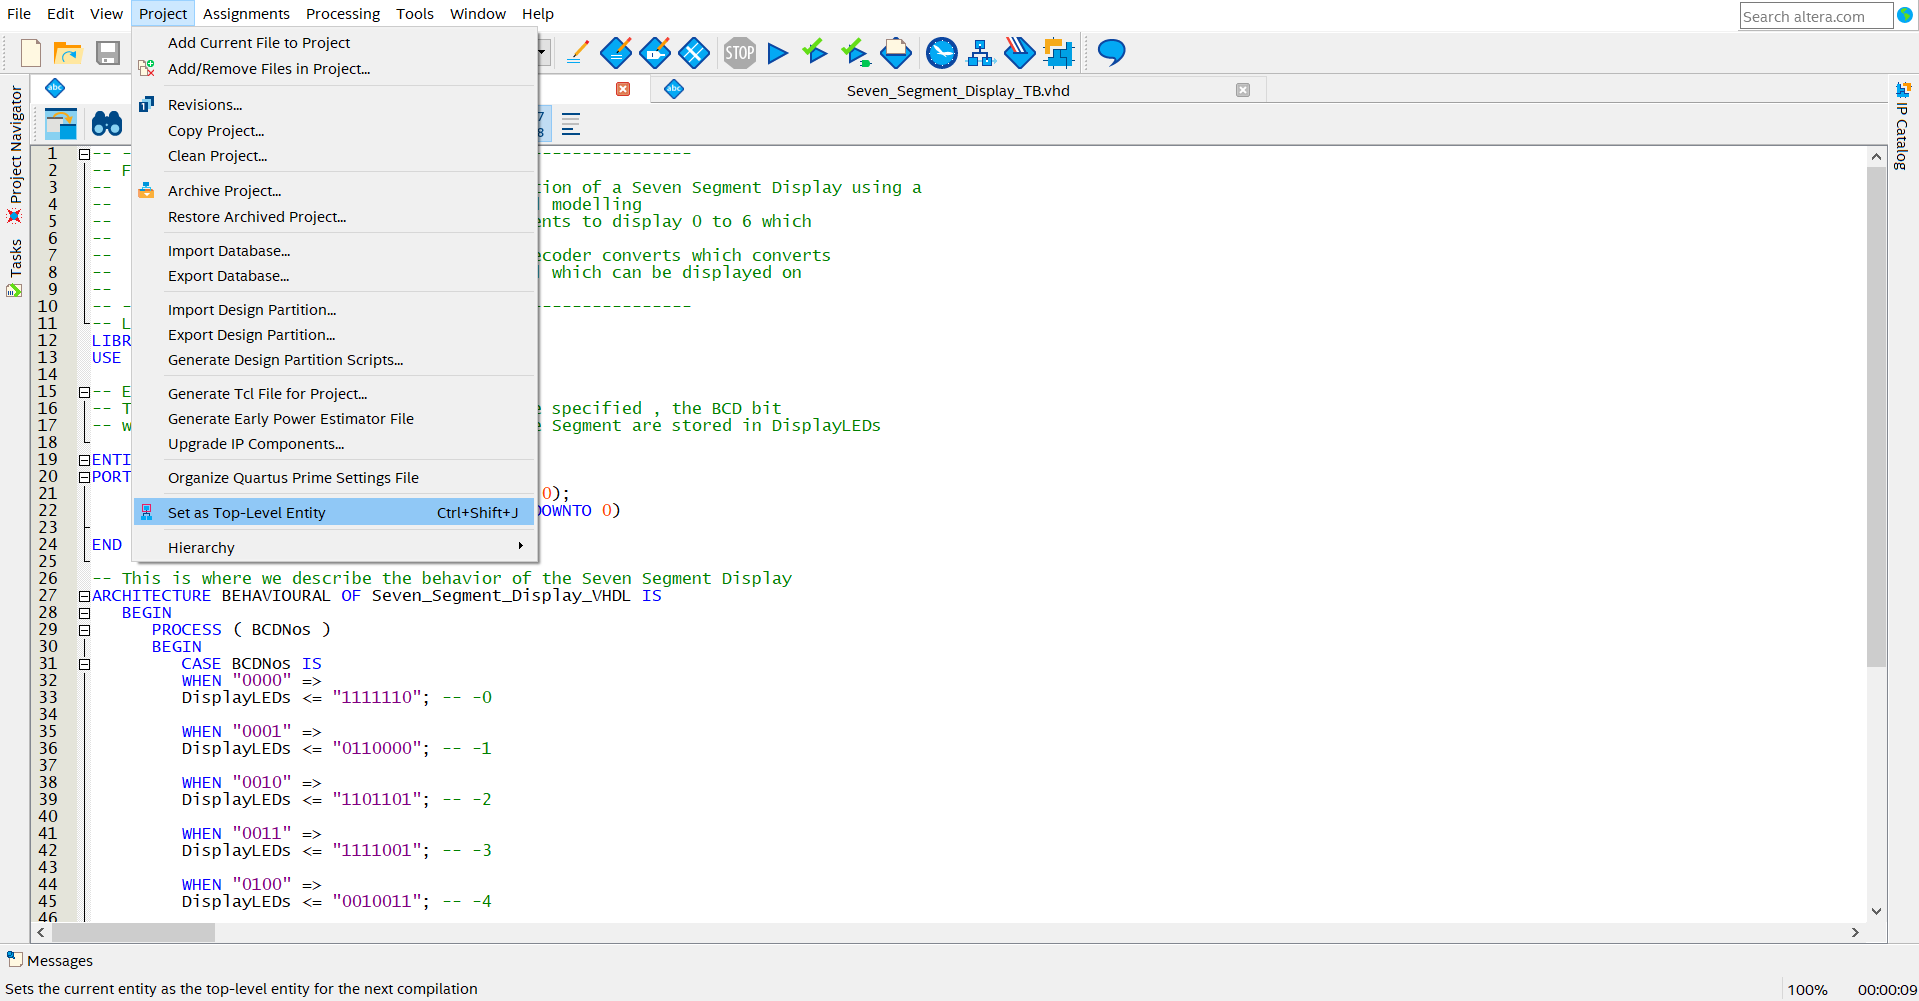
\includegraphics[width=14cm,keepaspectratio]{Project/Create4.png}
    \caption{Assign Top level Entity}
    \end{figure}
    \newpage
    \item Goto \textbf{Processing}$\rightarrow$\textbf{Start Compilation}. It takes sometime to complete. You can verify whether all the files are compiled successfully by checking the highlighted tabs i.e. \textbf{Messages} and \textbf{Tasks} tab.
    \begin{figure}[H]
    \centering
    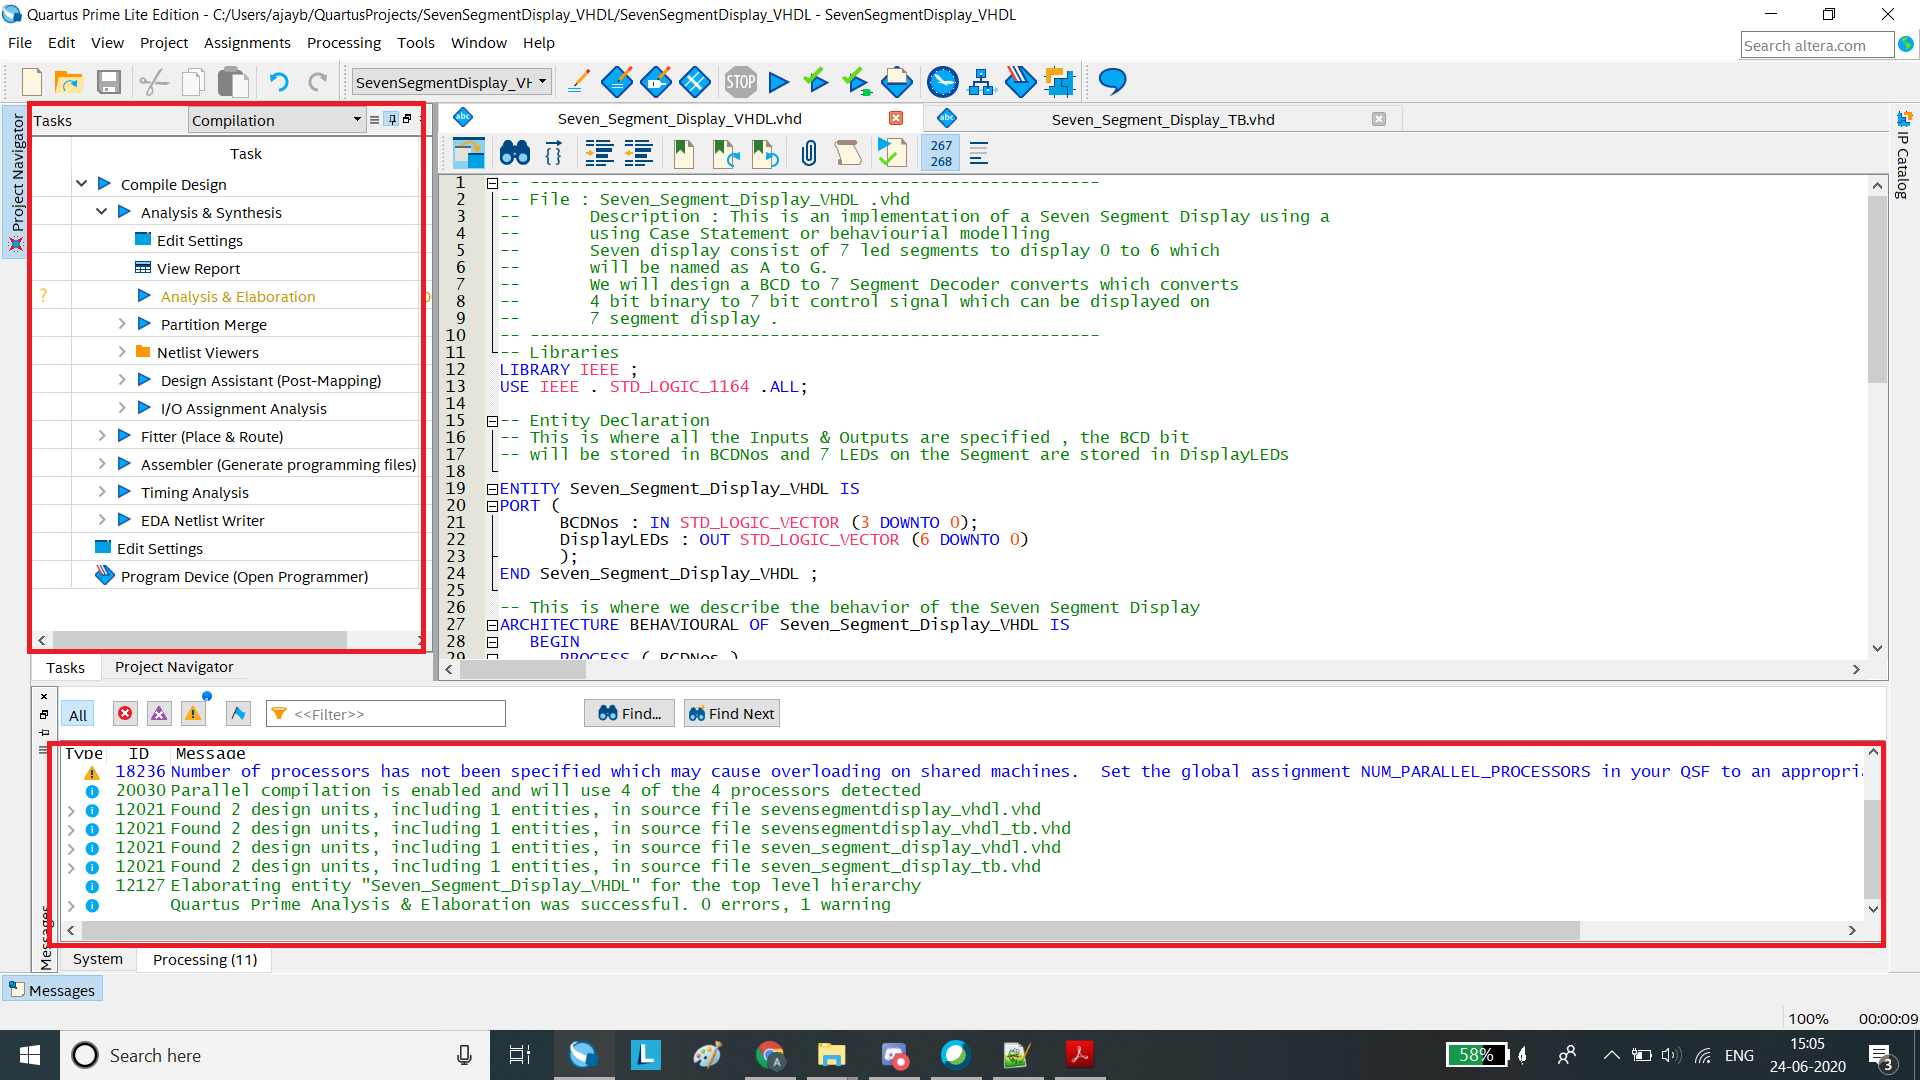
\includegraphics[width=12cm,keepaspectratio]{Project/Create5.png}
    \caption{Verification }
    \end{figure}
    
\end{enumerate}

\section{RTL Circuit of the implemented design}
The Figure shown in step 2 below shows the RTL design of the Seven Segment Display  circuit that we design using the above files. Here we can 7 select modules i.e 2:1 Muliplier, and one output and input block. The select lines for the Multiplier are from the 4-Bit DataBus input and the 7-Bit DataBus is the data line. If the input and the select lines matches for a particular Multiplier the the its 7 bit data is passed to the output.  
    \subsection*{Steps to get RTL circuit.}
    \vspace{4mm}
        
    \begin{enumerate}
            
        \item Goto \textbf{Tools}$\rightarrow$\textbf{Netlist Viewers}$\rightarrow$\textbf{RTL Viewer}.
        \vspace{6mm}
        \begin{figure}[H]
        \centering
        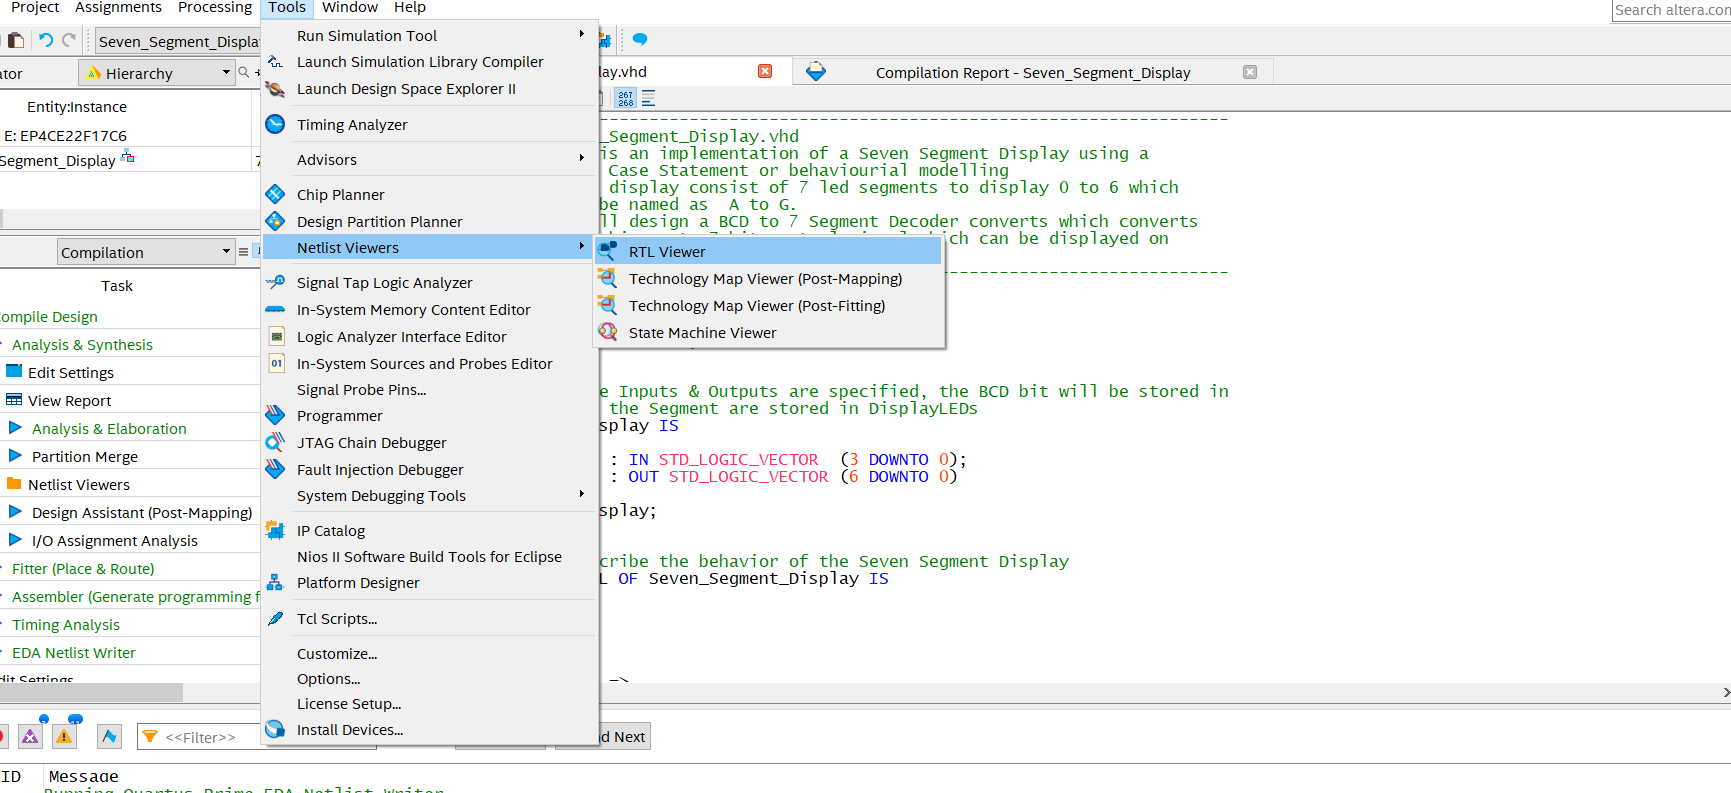
\includegraphics[width=14cm,keepaspectratio]{Project/Create6.png}
        \caption{Start RTL Viewer}
        \end{figure}
  \newpage      
        \item The below figure shows the equivalent RTL circuit of BCD decoder (4:7) or the design of Seven Segment Display using behavioral modelling.  \begin{figure}[H]
        \centering
        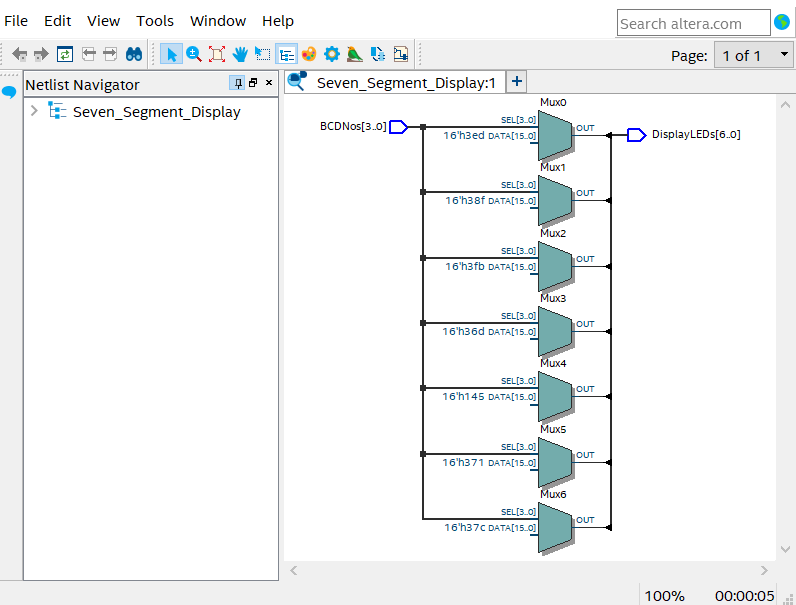
\includegraphics[width=12cm,keepaspectratio]{Project/Create7.png}
        \caption{RTL Design for Seven Segment Display}
        \end{figure}
    \end{enumerate}

\section{Pin  Assignment}
For in-depth guide for \textbf{Pin Assignment} a \textbf{New Project} follow \textbf{Quick Start Guide For Quartus Prime Lite Software Section 4.2}. This quide also contains a detailed pin description for DE0-Nano Board, so that you can select pin as per your requirement
    \begin{enumerate}

    \item Click on \textbf{Assignments}$\rightarrow$\textbf{Pin Planner},This Pin    Planner shows the I/O ports that we have created in our design.
    \begin{figure}[H]
    \centering
    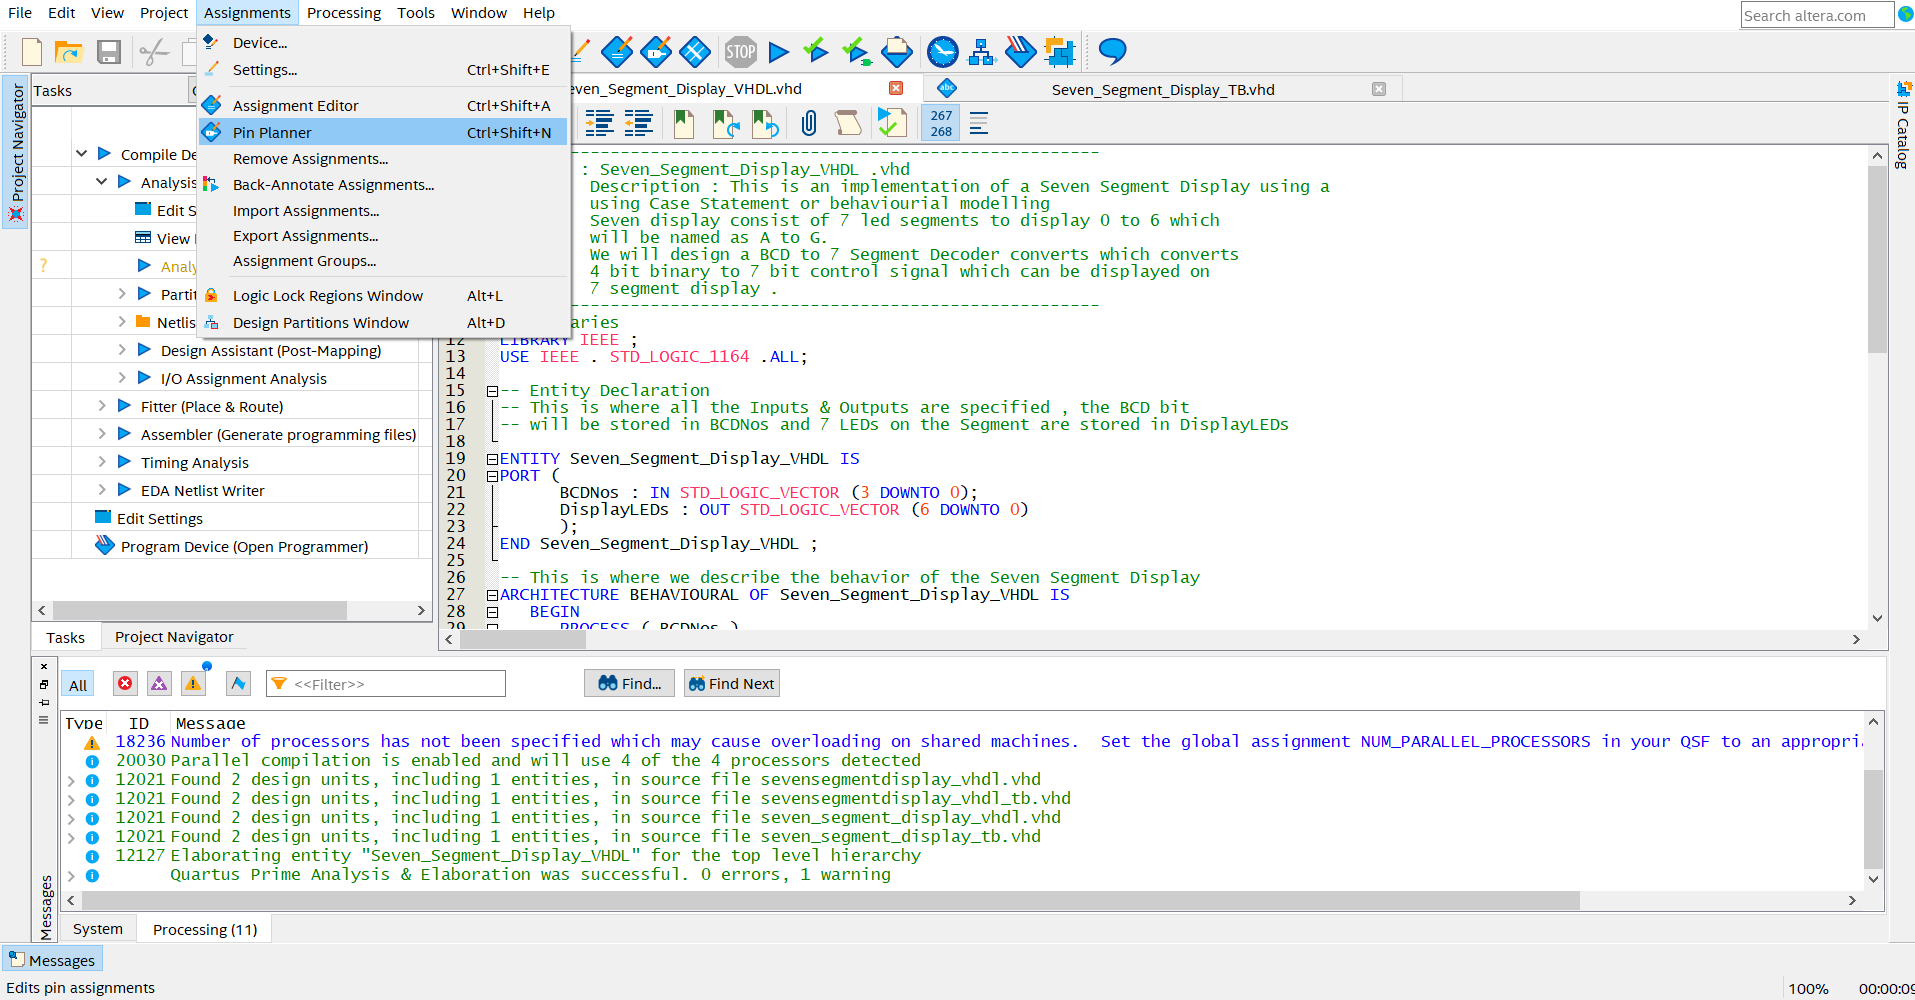
\includegraphics[width=14cm,keepaspectratio]{Project/Create8.png}
    \caption{Start Pin Planner}
    \end{figure}

    \item Now we have to assign each I/O ports with the respective Pin numbers, which can be found on the Device Manual which we are implementing.Here we are referring to the DEO NANO Board . If you a Seven Segment Display Module then you can use the GPIOs pins of the board and connect them to it. For this demonstration we will assign the \textbf{Output} to the LEDs[0 to 6] And assign all the \textbf{Inputs}(BCD) as the Slide Switch[0 to 3]
    \begin{center}
\begin{tabular}{ |p{3cm}|p{3cm}|p{3cm}|  } \hline
 \multicolumn{3}{|c|}{Pin Name for sliding Switches} \\ \hline \hline
Signal Name &   FPGA PinNo. &   Description         \\ \hline
DW[0]       &	PIN\_M1     &   BCDnos[0]   \\\hline
DW[1]       &	PIN\_T8      &   BCDnos[1]       \\\hline
DW[2]       &	PIN\_B9      &   BCDnos[3] 	    \\\hline
DW[3]       &	PIN\_M15      &   BCDnos[4]     \\\hline
\end{tabular}
\\
\begin{tabular}{ |p{3cm}|p{3cm}|p{3cm}| } \hline
 \multicolumn{3}{|c|}{Pin Name for LEDs} \\ \hline \hline
Signal Name &   FPGA PinNo. &   Description         \\ \hline
LED[0]       &	PIN\_A15         &   DisplayLEDs[0]      \\\hline
LED[1]       &	PIN\_A13        &   DisplayLEDs[1]      \\\hline
LED[2]       &	PIN\_B13         &   DisplayLEDs[2]	    \\\hline
LED[3]       &	PIN\_A11         &   DisplayLEDs[3]      \\\hline
LED[4]       &	PIN\_D1        &   DisplayLEDs[4]      \\\hline
LED[5]       &	PIN\_F3        &   DisplayLEDs[5]      \\\hline
LED[6]       &	PIN\_B1         &   DisplayLEDs[6]	    \\\hline
\end{tabular}
 \end{center}
    \begin{figure}[H]
    \centering
    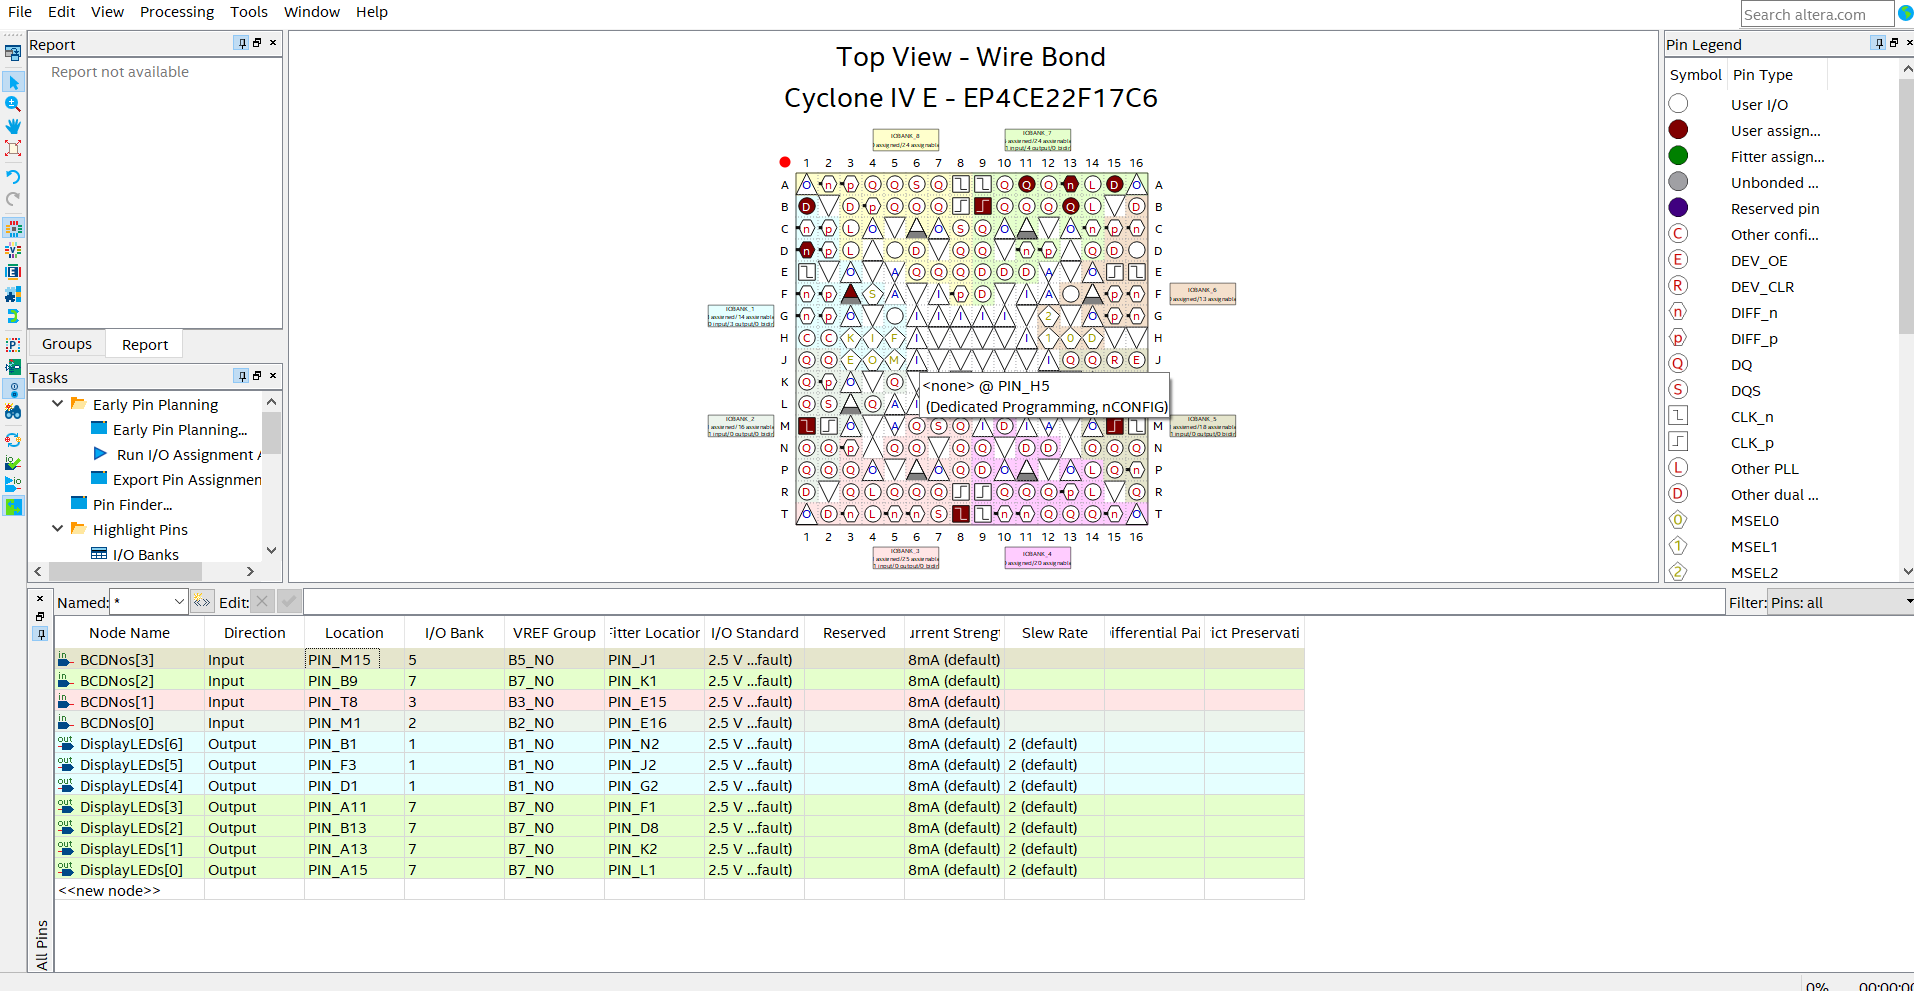
\includegraphics[width=14cm,keepaspectratio]{Project/Create9.png}
    \caption{Pin Assignment}
    \end{figure}

   \newpage 
    \item Go to \textbf{Processing}$\rightarrow$\textbf{Start I/O Assignment Analysis}. The analysis checks pin assignments and surrounding logic for illegal assignments and violations of board layout rules.
    \begin{figure}[H]
    \centering
    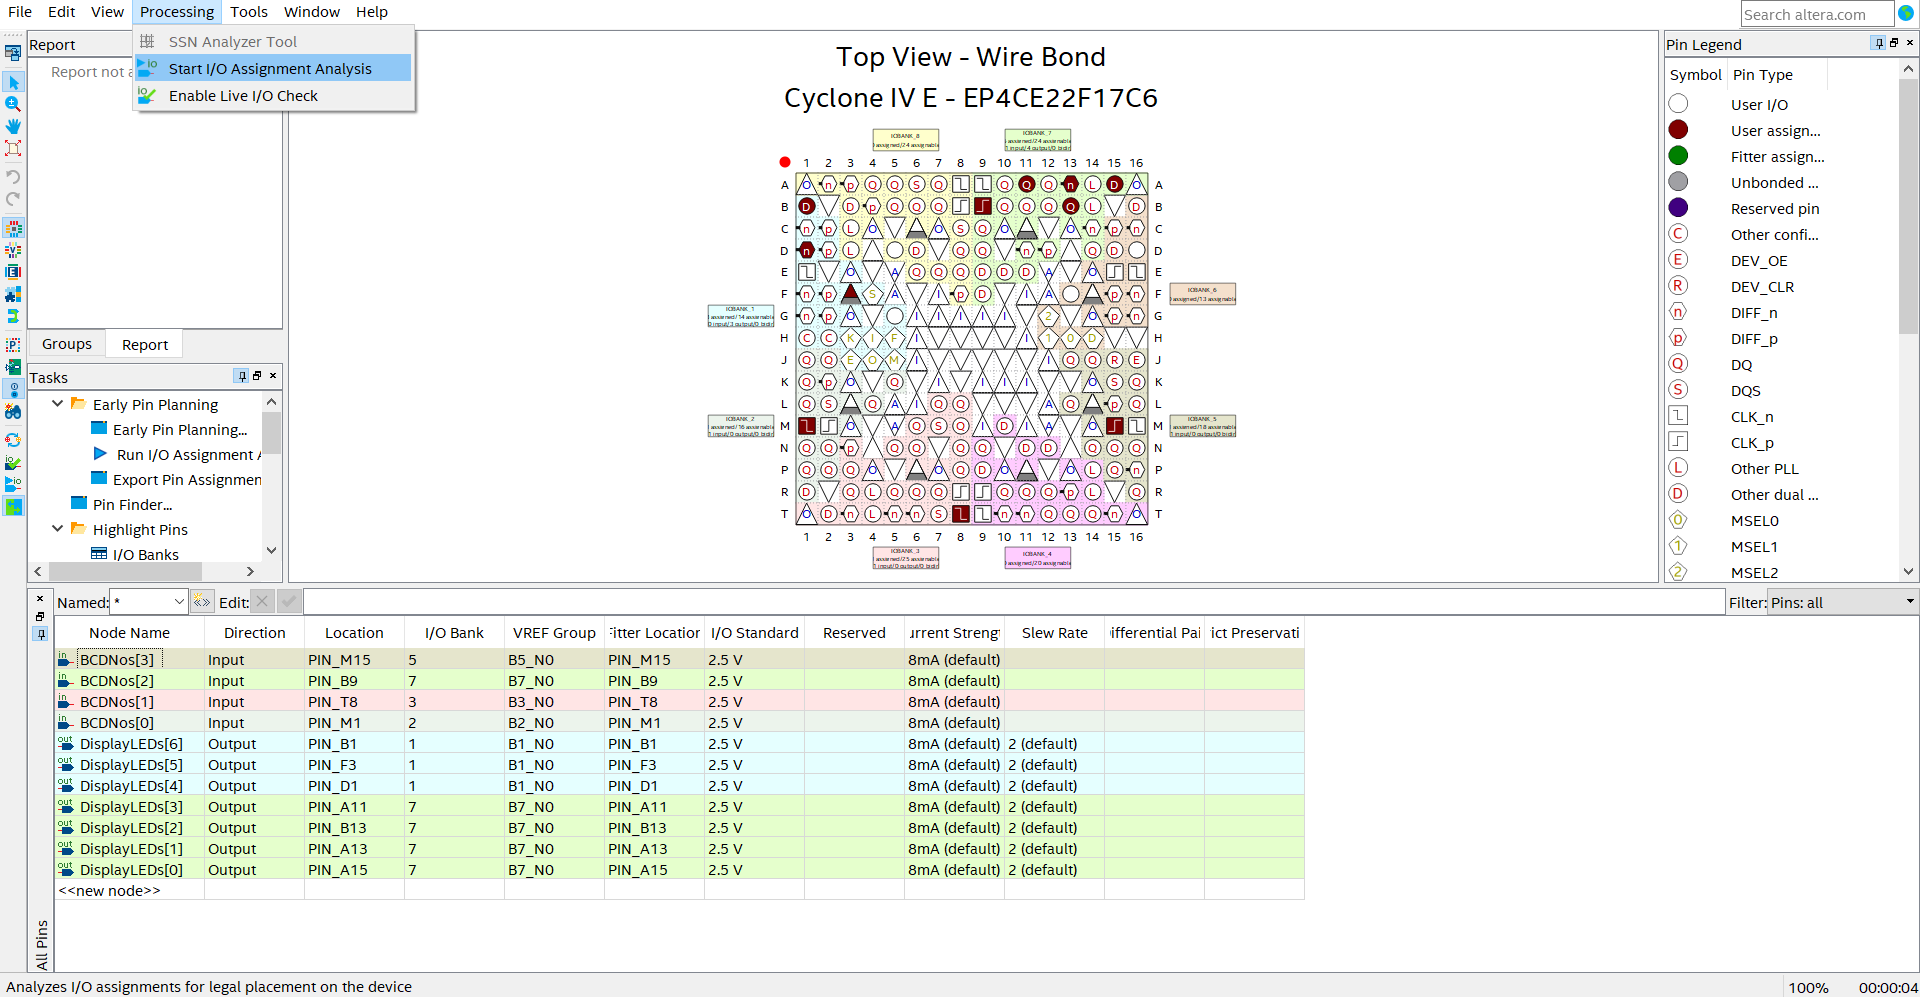
\includegraphics[width=12cm,keepaspectratio]{Project/Create10.png}
    \caption{Pin Analysis}
    \end{figure}
    
    \end{enumerate}

\section{Downloading the code to DE0 Nano FPGA Board}
Refer \textbf{Quick Start Guide to Quartus and ModelSim Software} \textbf{Section 4.3}.
The procedure to download the code to your FPGA board remains same, just make sure to \textbf{Compile} the correct file i.e \textbf{Seven\_Segment\_Display} which needs to be set as \textbf{Top Level Entity} while generating the .sof file.


\section{Implementing on Modelsim }
For more detailed procedure on using ModelSim, refer \textbf{Quick Start Guide to Quartus and ModelSim Software} Document. You can find both Verilog HDL and VHDL test bench code below, make sure to follow only one language in this entire tutorial.

 \begin{enumerate}
     \item Create a \textbf{New VHDL file}. Type in the Testbench code provided in this document and save the file with the same name as the module name
    \begin{figure}[H]
    \centering
    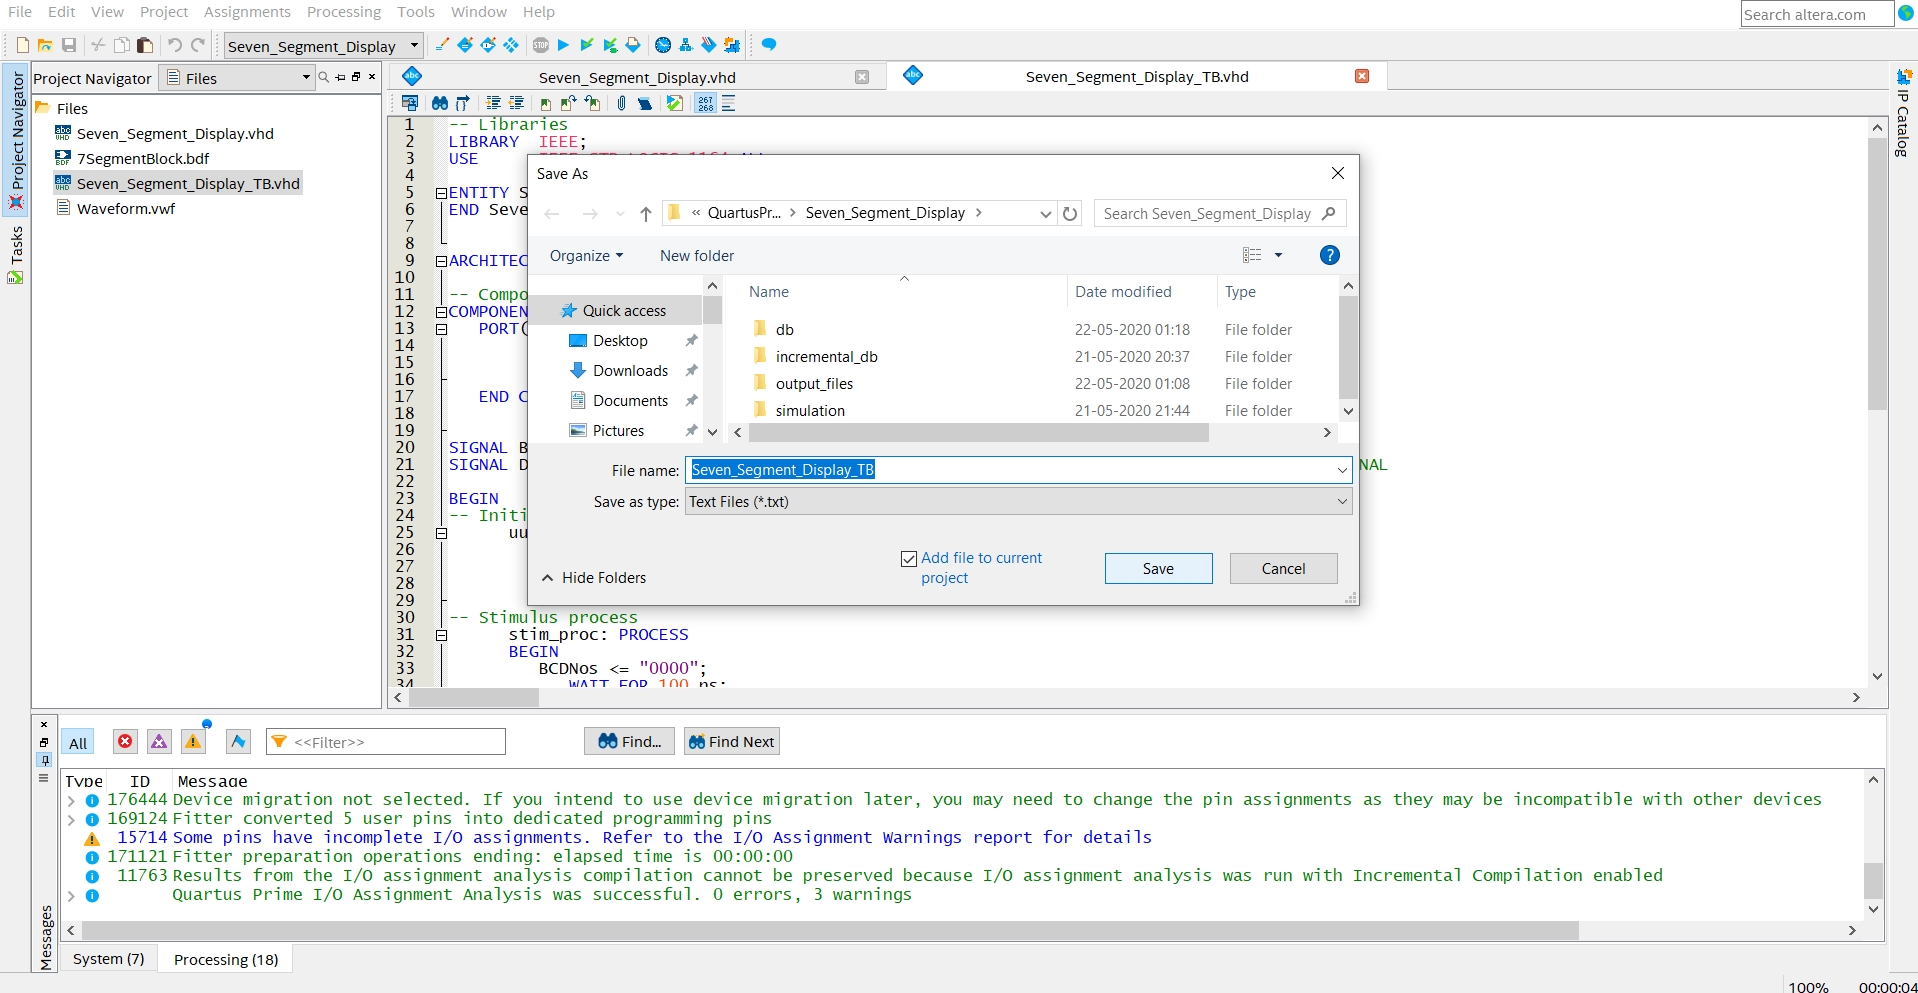
\includegraphics[width=12cm,keepaspectratio]{Project/Create11.png}
    \caption{Create a Test Bench}
    \end{figure}
   
    \item Go to \textbf{Assignments}$\rightarrow$\textbf{Settings}.
    
    \item Navigate to \textbf{Simulation} under \textbf{EDA Tool Settings}.Set the language as VHDL. Select \textbf{Compile Test Bench} and then click on \textbf{Test Benches}. You can find a detailed tutorial for setting a Test Bench file for simulation in the \textbf{Quick Start Guide to Quartus and ModelSim Software} Document in \textbf{\textbf{Section 5.2}}
    
    \item  Click on \textbf{Processing}$\rightarrow$\textbf{Start Compilation} 
    This process will check for any illegal statement occured in any of the files and give the error messages in the Messages section.
    
    
 \end{enumerate}
\subsection{Without TestBench}\\
 We can simulate our design without using a testbench file by using creating a \textbf{University Program VWF} file. You can find detailed steps to create and add Input and Output nodes in this files in the \textbf{Quick Start Guide to Quartus and ModelSim Software} Document in \textbf{Section 5.1}
  
\begin{enumerate}
    \item   Assign clock pulse to the inputs BCDNos[o to 3] as per the given table          and         run the simulation
            \begin{center}
    \begin{tabular}{ |p{3cm}|p{3cm}| } \hline
 \multicolumn{2}{|c|}{Clock Pulse For Inputs} \\ \hline \hline
\textbf{Input}      &       \textbf{Clock}         \\ \hline
DisplayLEDs[0]      &           50ns     \\\hline
DisplayLEDs[1]      &100ns\\\hline
DisplayLEDs[2]	    &200ns\\\hline
DisplayLEDs[3]      &     400ns  \\\hline

\end{tabular}        
  \end{center}
    \item   After running the simulation you can see the following results, also you can notice         for BCDNos "1010" to "1111" the output is zero because we mention the condition for         input greater than 9 the output in null or zero.
    
            \begin{figure}[H]
            \centering
            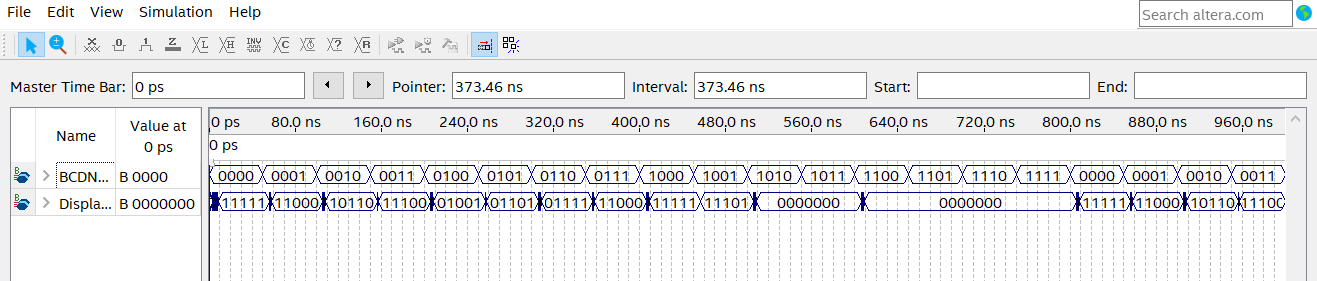
\includegraphics[width=14cm,keepaspectratio]{Simulation/Simulation5.png}
            \caption{Output Waveform}
            \end{figure}
            \newpage
            \textbf{Expanded form of above image}
            \begin{figure}[H]
            \centering
            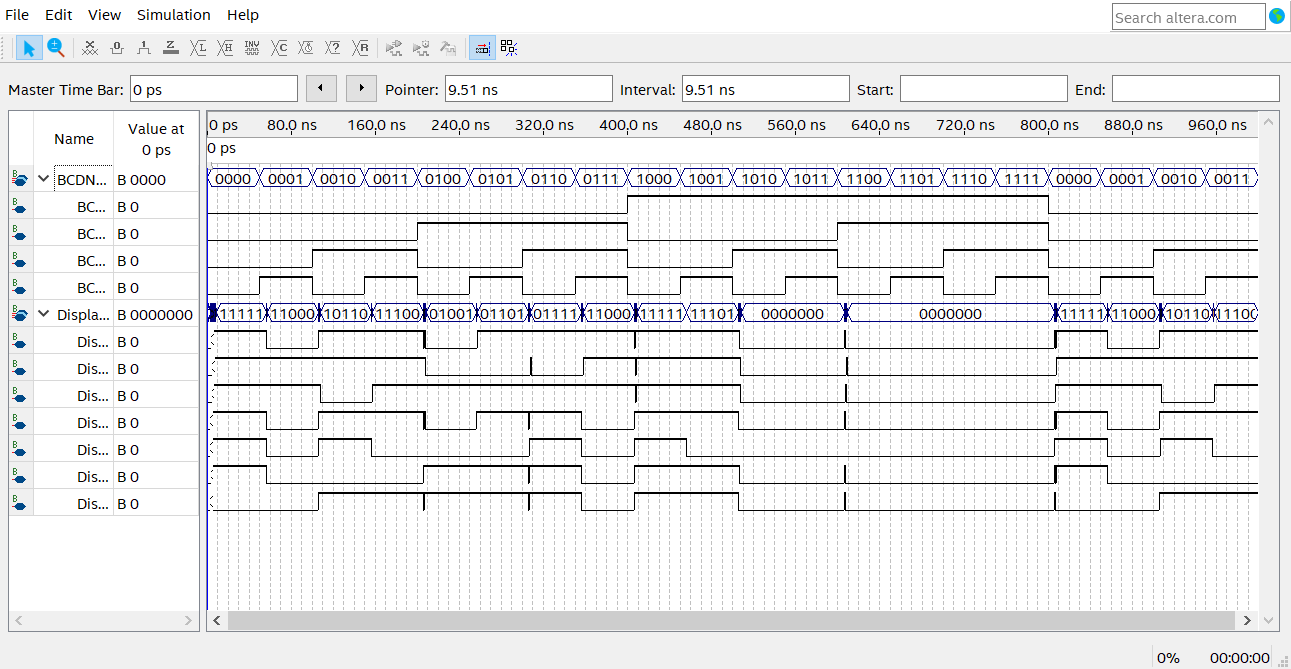
\includegraphics[width=14cm,keepaspectratio]{Simulation/Simulation6.png}
            \caption{Expanded Output Waveform}
            \end{figure}
            
    
\end{enumerate}
  
  

  
\subsection{Functional Simulation using NativeLink Feature}
    \begin{enumerate}
        
        \item Then Go to \textbf{Tools}$\rightarrow$\textbf{Run Simulation Tool}$\rightarrow$\textbf{RTL Simulation} to automatically run the EDA simulator(ModelSim-Altera) and to compile all necessary design files.
        \begin{figure}[H]
        \centering
        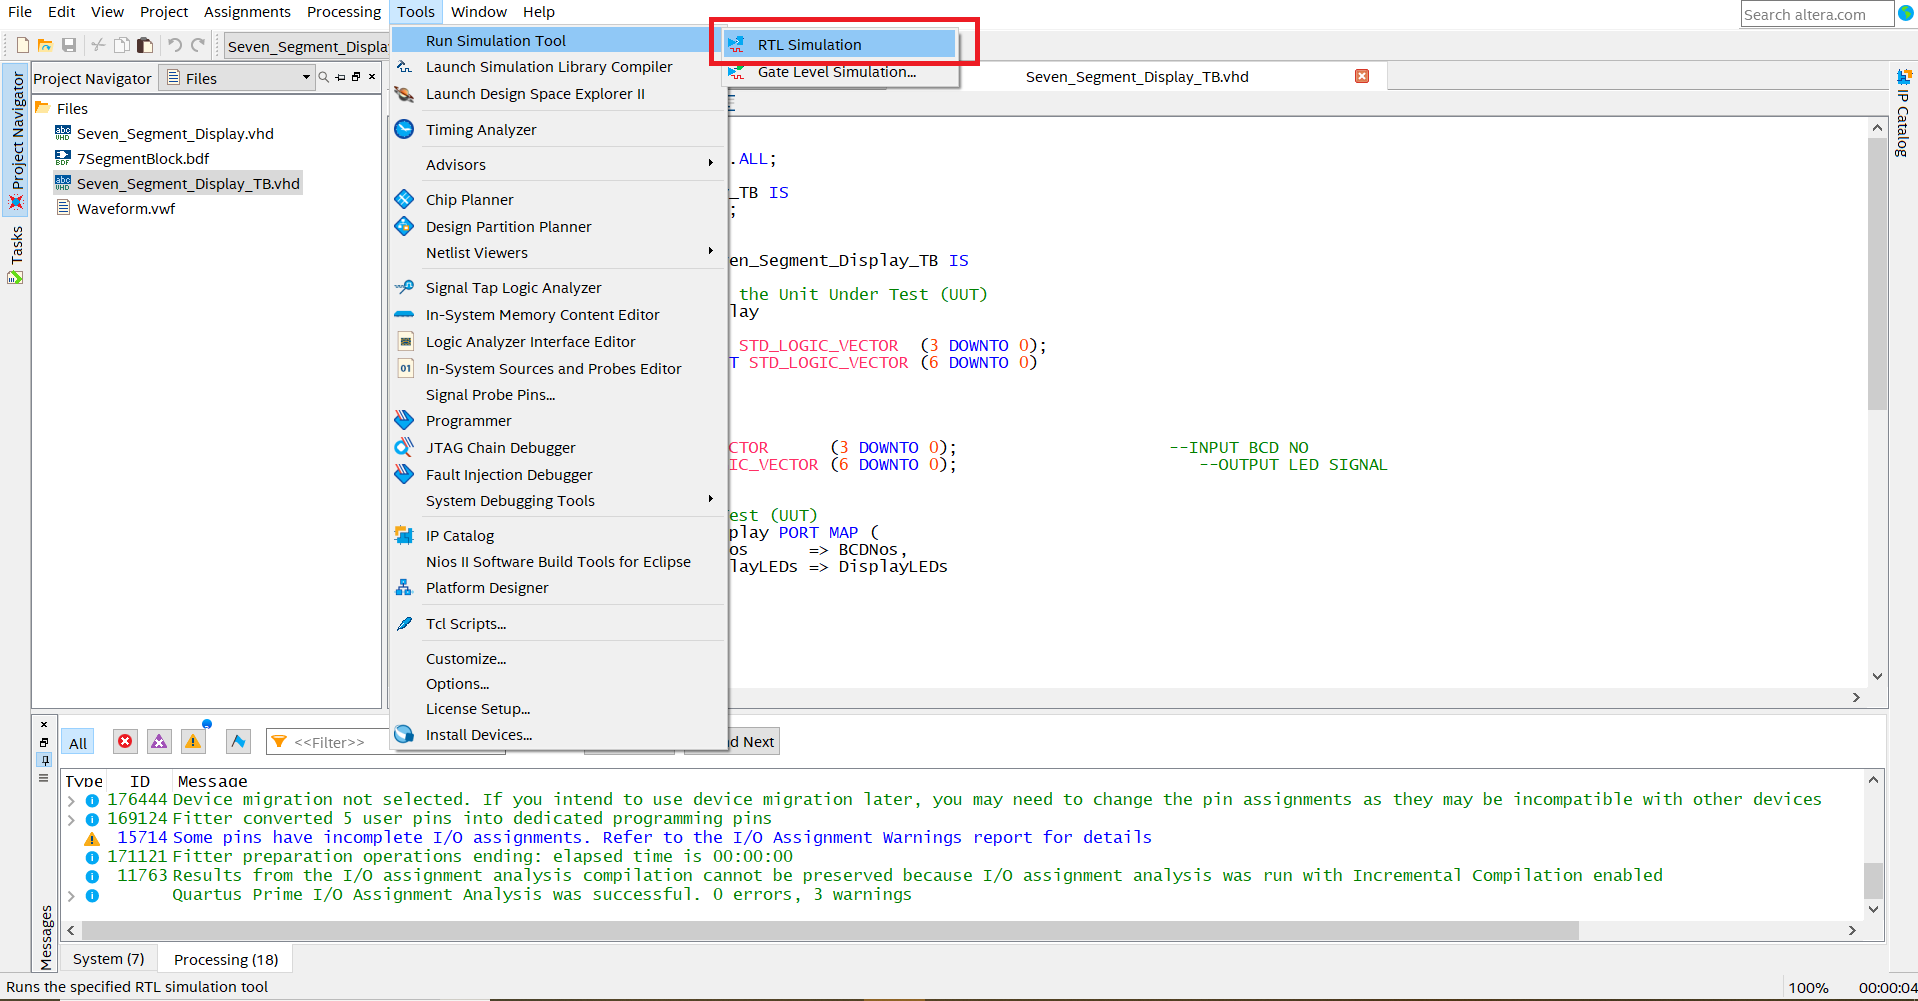
\includegraphics[width=14cm,keepaspectratio]{Simulation/Simulation1.png}
        \caption{Start RTL Simulation}
        \end{figure}

        \item Finally ModelSim-Altera tool opens,\\
        Add the I/O pins as shown in the below figure.
        Double click on the testbench file under 'Library' section,this adds the signals under 'Object' section.\\
        Start the simulation and add the test bench file.Then select all the signals (A , B and C) and add it to 'wave'section.
        \begin{figure}[H]
        \centering
        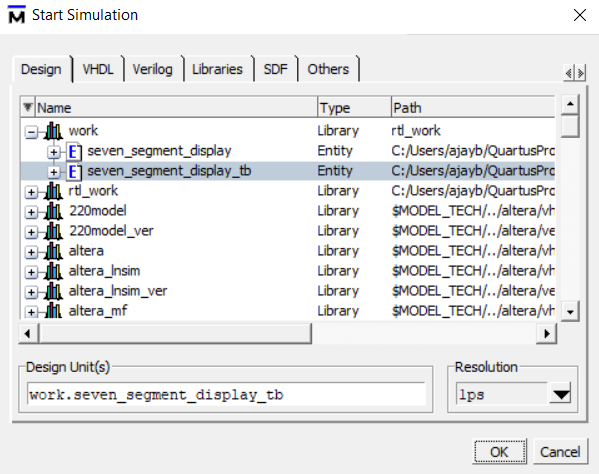
\includegraphics[width=8cm,keepaspectratio]{Simulation/Simulation2.png}
        \caption{Select TestBench file}
        \end{figure}
        \begin{figure}[H]
        \centering
        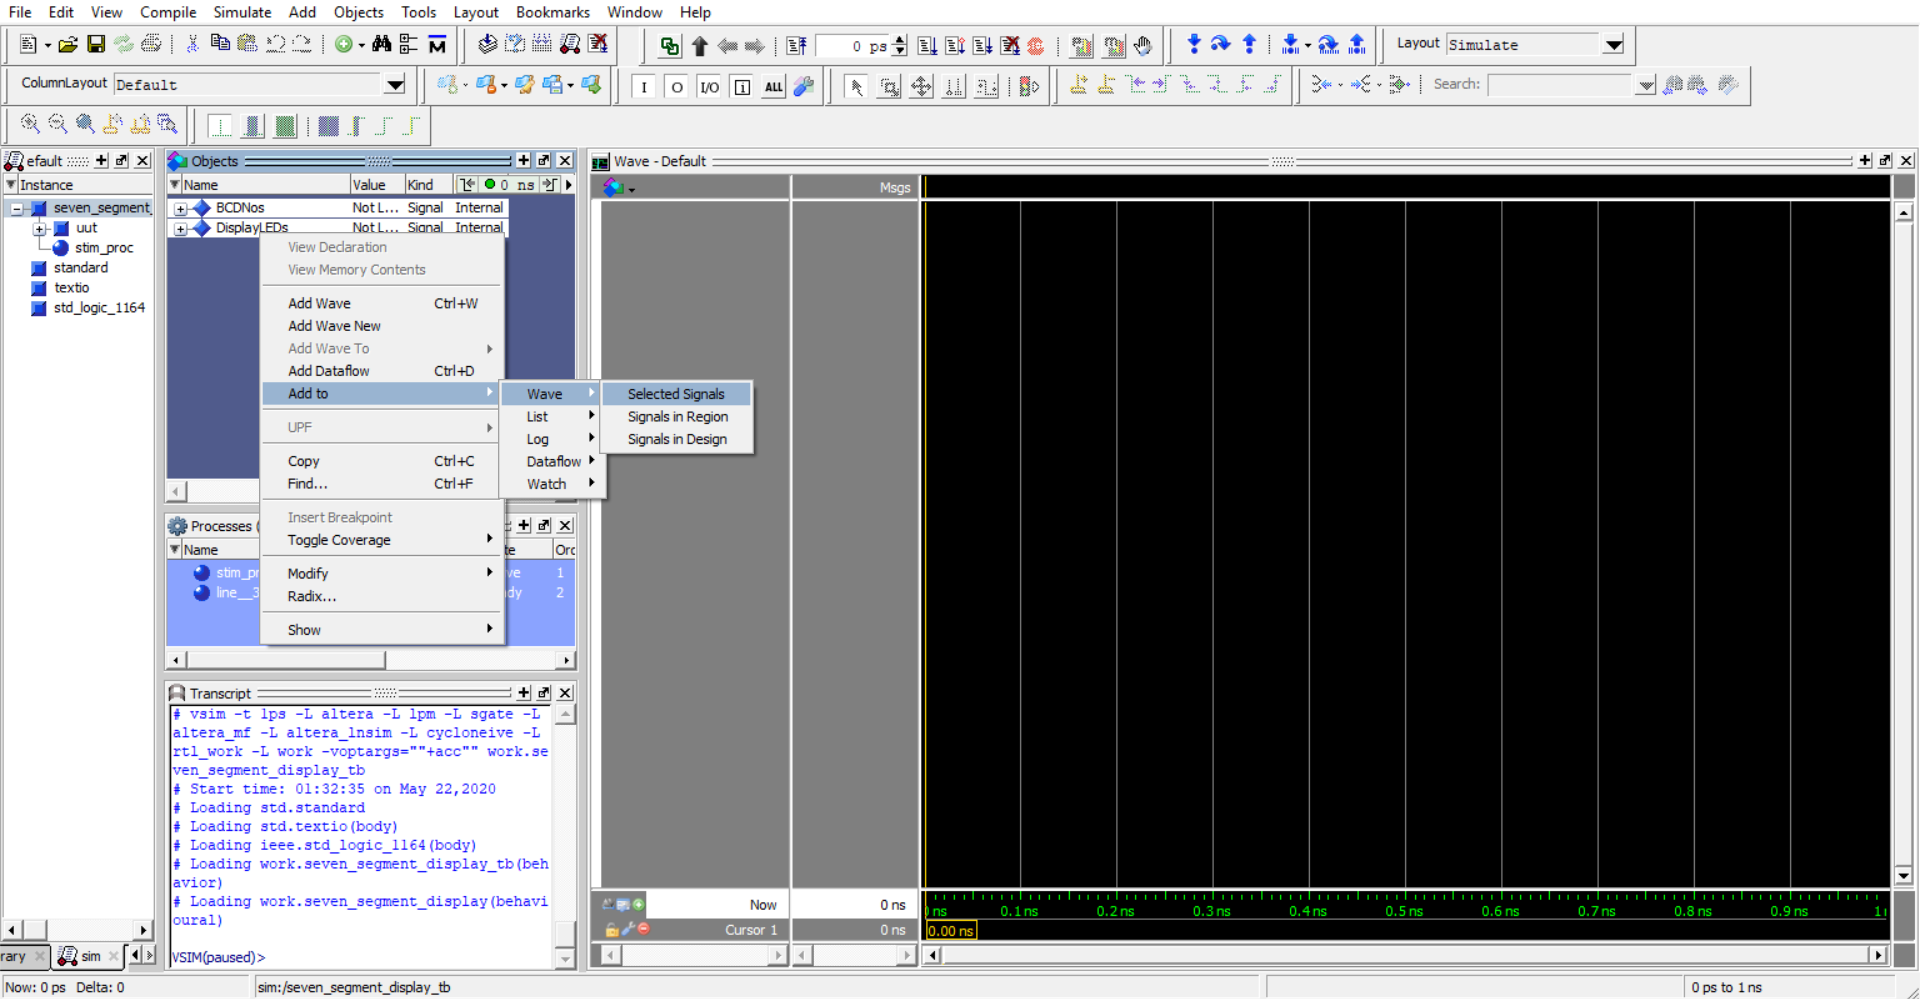
\includegraphics[width=11cm,keepaspectratio]{Simulation/Simulation3.png}
        \caption{Add I/O Signals}
        \end{figure}
        
        \item Start the simulation by clicking on the run all button in tool bar
        \begin{figure}[H]
        \centering
    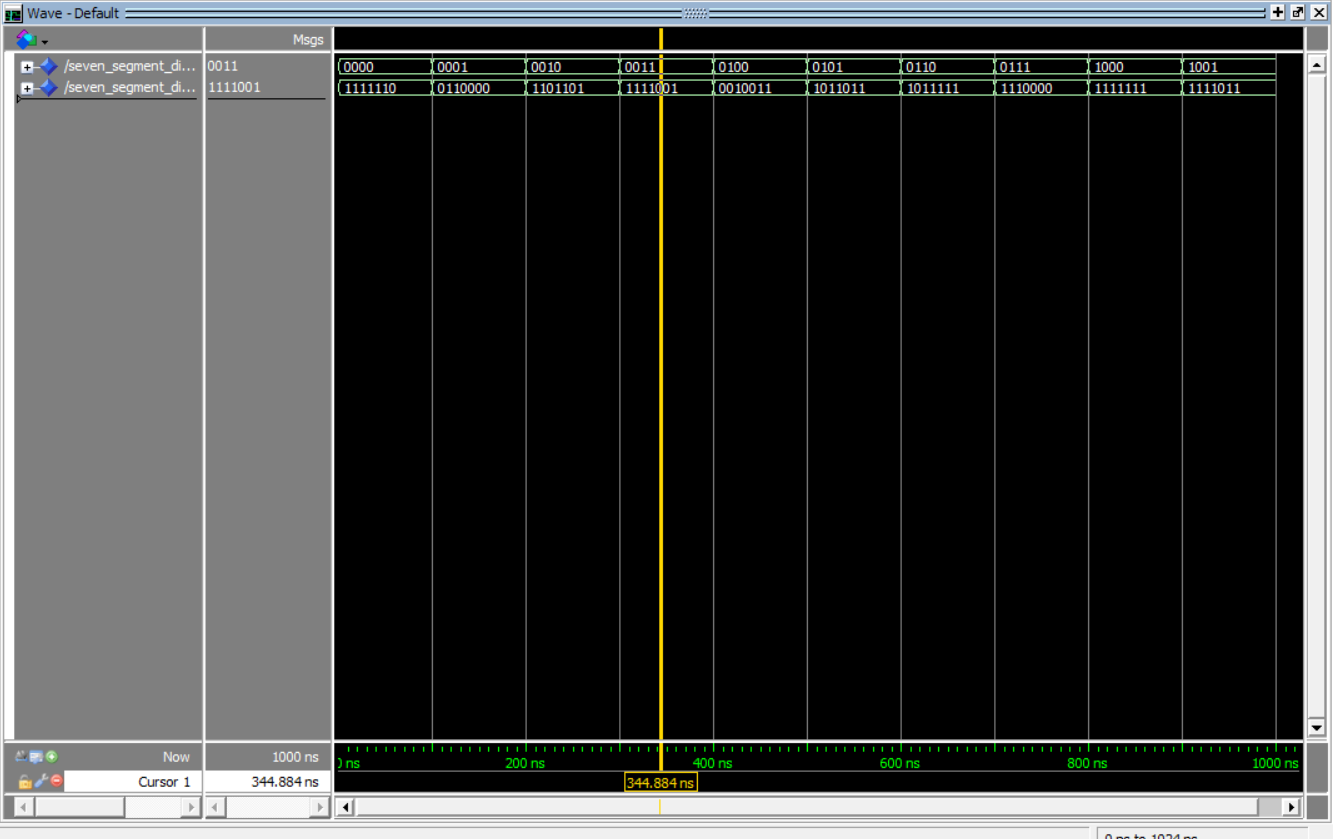
\includegraphics[width=11cm,keepaspectratio]{Simulation/Simulation4.png}
    \caption{Simulation}
    \end{figure}
    \item \textbf{Navigating the simulation }
    At this point you should have successfully run the simulation, but the waveform window is rather small and hard to see. 
    We can  move around in the simulation and see the value of the signals. Look for the cursor, a yellow vertical line in the waveform viewer, with the time in yellow at the bottom. You can use this line to move left or right in the waveform viewer and also zoom-in and zoom-out. 
    \end{enumerate}

\section{Testing the Design}

\subsection{Simulation waveform of our Design}
The Result shown below can be verified by comparing it with the Truth Table \\provided in page 2
    \begin{figure}[H]
    \centering
    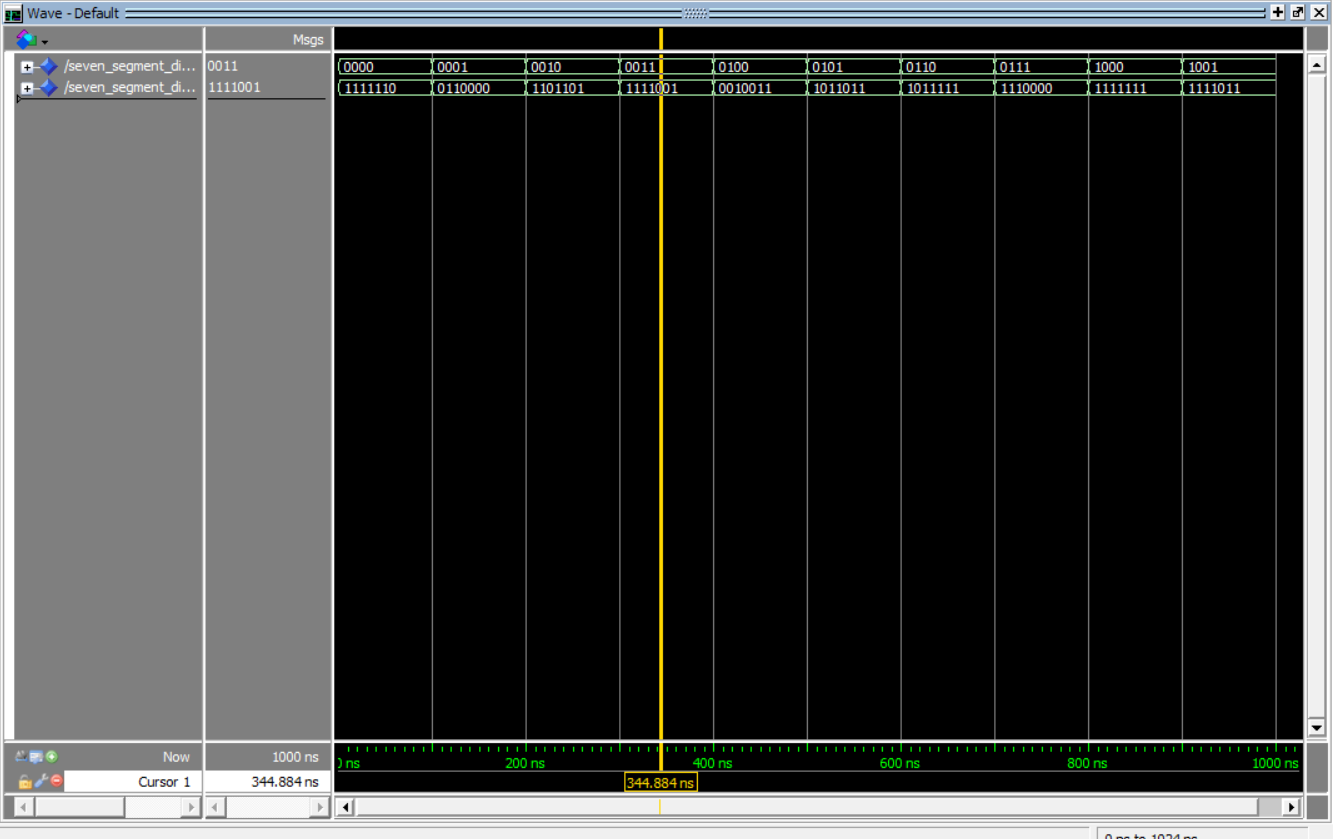
\includegraphics[width = 14cm,keepaspectratio]{Simulation/Simulation4.png}
    \caption{Final Output Waveform}
    \end{figure}
    
\noindent You can perform the same experiment using \textbf{Verilog HDL} language by using the code and testbench provided in code section of this document.


\end{document} 
 
